\documentclass{article}
\usepackage{fullpage}
\usepackage{amsmath}
\usepackage{amsfonts}
\usepackage{tipa}
\usepackage{tikz}
\newcommand\myeq{\mathrel{\stackrel{\makebox[0pt]{\mbox{\normalfont\tiny def}}}{=}}}
\begin{document}
\begin{center}
\Large{Hashtag Association}
\end{center} 
\vspace{.3cm} 
\par \indent
Autosegmental mapping from disjoint strings of tones and TBUs has been shown to be of a logical complexity greater than MSO in spite of its common use in analysis of autosegmental phenomena like tone (Jardine 2017). Enriching the representation to include morphological boundaries (\textit{hashtags}) on both tone and TBU tiers--and a binary relation between 
corresponding boundaries--shows promise in reining in the complexity of these mappings.
\section{Basic Architecture}
Consider for example a model in which tones and TBUs are separated by boundary markers.\\
\begin{center}
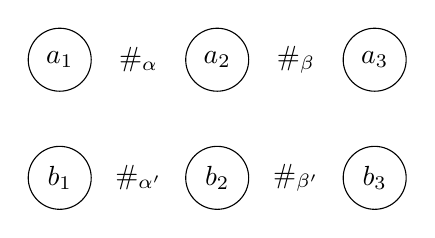
\begin{tikzpicture}
	\draw (-2,1.5) circle [radius = .4] node {$a_1$};
	\node at (-1,1.5) {$\#_{\alpha}$};
	\draw (0,1.5) circle [radius = .4] node {$a_2$};
	\node at (1,1.5) {$\#_{\beta}$};
	\draw (2,1.5) circle [radius = .4] node {$a_3$};
	\draw (-2,0) circle [radius = .4] node {$b_1$};
	\node at (-1,0) {$\#_{\alpha '}$};
	\draw (0,0) circle [radius = .4] node {$b_2$};
	\node at (1,0) {$\#_{\beta '}$};
	\draw (2,0) circle [radius = .4] node {$b_3$};
\end{tikzpicture}
\end{center}
In this representational schema, tautomorphemic tones and TBUs (e.g. $a_1$ and $b_1$) are separated from adjacent tones/TBUs by boundary markers in the autosegmental representation. There is no underlying association between tones and TBUs that belong to the same morpheme; there is, however, a relationship between boundary markers across tiers. A relation (though not necessarily \textit{association} in the traditional sense) exists between morpheme markers across tiers that share edges with tautomorphemic tones/TBUs ($\#_{\alpha}$ and $\#_{\alpha '}$ in the above example, for instance). Within a particular model, this is represented as a binary relation which constitutes part of the input signature. The model above, for example, can be described by the input signature
\smallskip{}
\begin{center}
$\langle D; \triangleleft, P_{a}, P_{b}, P_{\#}, R_{\#}, \rangle$
\end{center}
such that $R_{\#} \in  \{ (\#_{\alpha}, \#_{\alpha '}), (\#_{\beta}, \#_{\beta '}) \}$. These boundaries are ordered with respect to other elements on their designated tier. As such, the output association relation is expressed largely in terms of this ordering. Examples in the following section illustrate.
\section{Examples}
Using the morpheme boundary formalism and the example model above, a basic one-to-one, left-to-right association relation ($\circ$) is defined as follows:
\begin{center}
$x \circ y \myeq  \exists z, v[x \triangleleft z  \wedge  y \triangleleft v  \wedge  R_{\#}(z, v)]$
\end{center}
The variables $z$ and $v$ in the definition correspond to morpheme boundaries on the tonal and TBU tiers. A tonal-tier segment ($x$) will immediately precede a morpheme boundary ($z$); that boundary is in the $R_{\#}$ relation with a corresponding boundary on the TBU tier ($v$), which is the successor to a corresponding TBU ($y$). As defined, this association relation can associate tones and TBUs rightward in an unbounded fashion.
\begin{center}
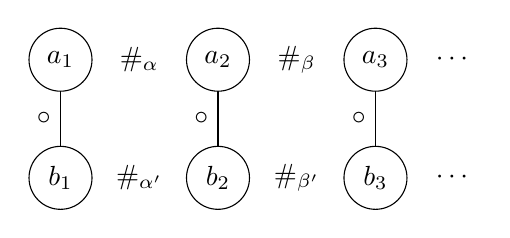
\begin{tikzpicture}
	\draw (-2,1.5) circle [radius = .4] node {$a_1$};
	\node at (-1,1.5) {$\#_{\alpha}$};
	\draw (0,1.5) circle [radius = .4] node {$a_2$};
	\node at (1,1.5) {$\#_{\beta}$};
	\draw (2,1.5) circle [radius = .4] node {$a_3$};
	\draw (-2,0) circle [radius = .4] node {$b_1$};
	\node at (-1,0) {$\#_{\alpha '}$};
	\draw (0,0) circle [radius = .4] node {$b_2$};
	\node at (1,0) {$\#_{\beta '}$};
	\draw (2,0) circle [radius = .4] node {$b_3$};
	\node at (3,1.5) {$\dotsb$};
	\node at (3,0) {$\dotsb$};
	\draw [-] (-2,1.1) -- (-2,.4) node [left, pos = .5] {$\circ$};
	\draw [-] (0,1.1) -- (0,.4) node [left, pos = .5] {$\circ$};
	\draw [-] (2,1.1) -- (2,.4) node [left, pos = .5] {$\circ$};
\end{tikzpicture}\\
\end{center}
A Kikuyu-type tone shift pattern can also be represented within this framework. The output association relation is defined in a way similar to above, with the addition of conjuncts utilizing $\varphi_{\mathsf{initial}}$ and $\varphi_{\mathsf{final}}$ predicates (to mirror the WFC3 and High Tone Association rules respectively; see Clements and Ford 1979).
\begin{center}
$x \circ y \myeq \exists z, v[z \triangleleft x  \wedge  y \triangleleft v  \wedge  R_{\#}(z, v)] \lor [\mathsf{initial}(x) \wedge \mathsf{initial}(y)] \lor [\mathsf{final}(x) \wedge \mathsf{final}(y)]$
\end{center}
The first conjunct in this definition is almost identical to that for L-to-R association, with the single exception that instead of the morpheme boundary ($v$) as successor to the TBU ($y$), the inverse order obtains. This yields association one TBU to the right (hence the tone-shift effect), as below.
\begin{center}
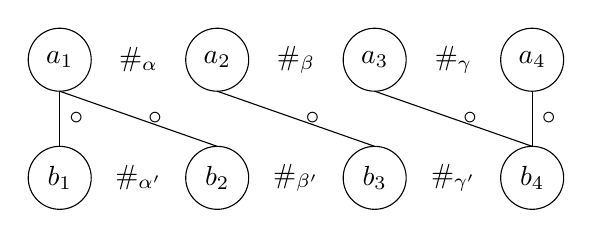
\begin{tikzpicture}
	\draw (-2,1.5) circle [radius = .4] node {$a_1$};
	\node at (-1,1.5) {$\#_{\alpha}$};
	\draw (0,1.5) circle [radius = .4] node {$a_2$};
	\node at (1,1.5) {$\#_{\beta}$};
	\draw (2,1.5) circle [radius = .4] node {$a_3$};
	\node at (3,1.5) {$\#_{\gamma}$};
	\draw (4,1.5) circle [radius =.4] node {$a_4$};
	\draw (-2,0) circle [radius = .4] node {$b_1$};
	\node at (-1,0) {$\#_{\alpha '}$};
	\draw (0,0) circle [radius = .4] node {$b_2$};
	\node at (1,0) {$\#_{\beta '}$};
	\draw (2,0) circle [radius = .4] node {$b_3$};
	\node at (3,0) {$\#_{\gamma '}$};
	\draw (4,0) circle [radius=.4] node {$b_4$};
	\draw [-] (-2,1.1) -- (-2,.4) node [right, pos = .5] {$\circ$};
	\draw [-] (4,1.1) -- (4,.4) node [right, pos = .5] {$\circ$};
	\draw [-] (-2,1.1) -- (0,.4) node [right, pos = .5] {$\circ$};
	\draw [-] (0,1.1) -- (2,.4) node [right, pos = .5] {$\circ$};
	\draw [-] (2,1.1) -- (4,.4) node [right, pos = .5] {$\circ$};
\end{tikzpicture}
\end{center}
Important to note here is that the same morpheme boundary pair is used as a reference point in both definitions to achieve rather different effects.
\section{Residual Issues}
Some issues remain with these characterizations.  Chief among these is the question of whether the morpheme boundaries are motivated theoretically and/or empirically. In other words, is there a motivation for this analysis which makes it more parsimonious than simply positing underlying associations between tautomorphemic tones and TBUs? This leads to related questions about where they (should/are motivated to) exist. Is each tone/TBU pair within a morpheme wrapped in morpheme boundaries? Are the boundaries assumed to be part of lexical representation for the morphemes or is there some derivational process in which morphemes are concatenated, after which boundaries are placed between them?
So far, the analysis has only dealt with cases in which each morpheme comprises a single tone and single TBU. What about cases of tonal morphemes, where a morpheme contains a tone but not a TBU? Association in such cases is not problematic when the tonal morpheme appears string-finally, but the answer less straight-forward when it appears in the middle of a string (see the examples below).
\begin{center}
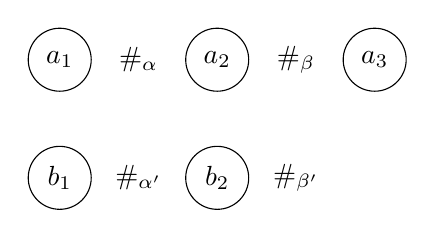
\begin{tikzpicture}
	\draw (-2,1.5) circle [radius = .4] node {$a_1$};
	\node at (-1,1.5) {$\#_{\alpha}$};
	\draw (0,1.5) circle [radius = .4] node {$a_2$};
	\node at (1,1.5) {$\#_{\beta}$};
	\draw (2,1.5) circle [radius = .4] node {$a_3$};
	\draw (-2,0) circle [radius = .4] node {$b_1$};
	\node at (-1,0) {$\#_{\alpha '}$};
	\draw (0,0) circle [radius = .4] node {$b_2$};
	\node at (1,0) {$\#_{\beta '}$};
\end{tikzpicture}
\hspace{1.5cm}
vs.
\hspace{1.5cm}
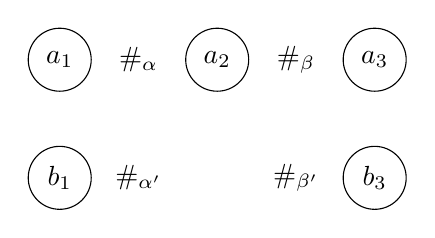
\begin{tikzpicture}
	\draw (-2,1.5) circle [radius = .4] node {$a_1$};
	\node at (-1,1.5) {$\#_{\alpha}$};
	\draw (0,1.5) circle [radius = .4] node {$a_2$};
	\node at (1,1.5) {$\#_{\beta}$};
	\draw (2,1.5) circle [radius = .4] node {$a_3$};
	\draw (-2,0) circle [radius = .4] node {$b_1$};
	\node at (-1,0) {$\#_{\alpha '}$};
	\node at (1,0) {$\#_{\beta '}$};
	\draw (2,0) circle [radius = .4] node {$b_3$};
\end{tikzpicture}
\end{center}
Another issue concerns language which exhibit the inverse pattern: multiple tonal segments per TBU or contour tones. Under the current analysis, a contour tone on the melodic tier would be realized as (at least) two tonal segments followed by a morpheme boundary. How, then, to define the association relation below, without assuming underlying association?
\begin{center}
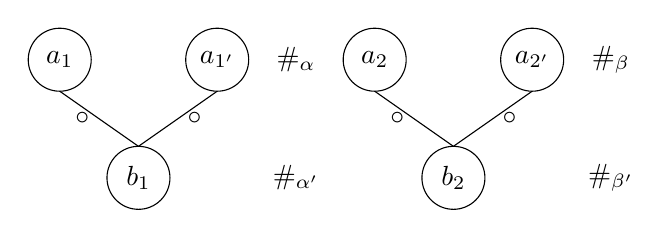
\begin{tikzpicture}
	\draw (-2,1.5) circle [radius = .4] node {$a_1$};
	\draw (0,1.5) circle [radius = .4] node {$a_{1'}$};
	\node at (1,1.5) {$\#_{\alpha}$};
	\draw (2,1.5) circle [radius = .4] node {$a_2$};
	\draw (4,1.5) circle [radius =.4] node {$a_{2'}$};
	\draw (-1,0) circle [radius = .4] node {$b_1$};
	\node at (1,0) {$\#_{\alpha '}$};
	\node at (5,1.5) {$\#_{\beta}$};
	\node at (5,0) {$\#_{\beta '}$};
	\draw (3,0) circle [radius = .4] node {$b_2$};
	\draw [-] (-2,1.1) -- (-1,.4) node [left, pos = .5] {$\circ$};
	\draw [-] (0,1.1) -- (-1,.4) node [right, pos = .5] {$\circ$};
	\draw [-] (2,1.1) -- (3,.4) node [left, pos = .5] {$\circ$};
	\draw [-] (4,1.1) -- (3,.4) node [right, pos = .5] {$\circ$};
\end{tikzpicture}
\end{center}
At first glance, it seems possible that the precedence relation (<) could supplant successor ($\triangleleft$) in the association definition. Such a definition looks rather similar to the one-to-one, L-to-R definition discussed above:
\begin{center}
$x \circ y \myeq  \exists z, v[x < z \wedge y < v \wedge R_{\#}(z, v)]$
\end{center}
This definition, for example, would allow both $a_1$ and $a_{1'}$ to association to $b_1$, given the nature of the precedence relation. This is the desired effect. However, the definition is insufficient in its restrictiveness; it produces the unwanted effect of allowing $a_2$ and $_{2'}$ to associate to $b_1$ as well. Limiting association to the substring which falls \textit{between} two boundaries will need to be worked out.
\pagebreak
\begin{center} References \end{center}
\smallskip{}
\hangindent=.5cm
Clements, George and Kevin Ford. 1979. Kikuyu tone shift and its synchronic consequences. \textit{Linguistic Inquiry} 10,2: 197-210.\\
\par \noindent
\hangindent=.5cm
Jardine, Adam. 2017. On the logical complexity of autosegmental representations. \textit{Proceedings of the 15th Meeting on the Mathematics of Language}: 22-35.\\
\end{document}